\documentclass[dvipdfmx]{jsarticle}
% \usepackage{subfigure}
\usepackage{graphicx}
\usepackage{multicol}
\usepackage{float}
\usepackage{circuitikz}
\usepackage{tikz}
\usepackage{amssymb}
\usepackage{arydshln}
\usepackage{wrapfig}
\usepackage{url}
\usepackage{amsmath}
% \usepackage{mathtools}
\usepackage{Tabbing}
\usepackage{footnote}
% \usepackage{currfile}
% \usepackage{fancyhdr}

\newcommand{\undercolor}[2][orange]{
  \textcolor{#1}{\underline{\textcolor{black}{#2}}}
}

\newlength{\tabpos}
\newlength{\remainwidth}

\newcommand{\measuretab}[1]{%
  \settowidth{\tabpos}{#1}%
  \global\setlength{\remainwidth}{\textwidth}
  \global\addtolength{\remainwidth}{-\tabpos}
}

\newcommand{\wraptab}[1]{
  \parbox[t]{\remainwidth}{#1}
}


\pagestyle{headings}
% \pagestyle{plain}
% \renewcommand{\headrulewidth}{0pt}
% \fancyfoot[L]{\currfilename}
\begin{document}
% \thispagestyle{fancy}
\markboth{\jobname}{\jobname}
\title{コンピュータネットワーク}
\date{}
\author{}
\maketitle

\section{コンピュータネットワーク概観}

\subsection{コンピュータネットワークの構成}

\subsubsection{インターネットの構成}

\begin{itemize}
  \item エンドシステム (end system)
  \begin{itemize}
    \item ネットワークに接続しているコンピュータ
    \item ホストともいう
    \item クライアントとサーバに分類されることが多い
  \end{itemize}
  \item クライアント\\
    サービス要求を出す
  \item サーバ\\
    サービス要求を待ち受ける
  \item 通信リンク\\
    光ファイバ、電波、同軸ケーブル、etc...
  \item ルータ\\
    パケットの中継装置
  \item \textcolor{cyan}{ここまでがモノ}
  \item プロトコル\\
    二つ以上の通信エンティティ間でやりとりされるメッセージの形式と順序などを取り決める規約\\
    \textcolor{cyan}{ネットワークの機器間でのやり取りにおけるルール}
\end{itemize}

\newpage
\subsubsection{通信サービス}

エンドシステム間で情報をやり取りするための仕掛け
\begin{itemize}
  \item \textcolor{orange}{コネクション指向型サービス}\\
    クライアントとサーバは、通信を始める前に相互に制御パケットを送信\\
    \textcolor{cyan}{通信前にハンドシェイク}
    \begin{itemize}
      \item \textcolor{orange}{高信頼データ転送}\\
        順序通り、誤りなく伝送
      \item \textcolor{orange}{フロー制御}\\
        受信側のバッファを溢れさせない\\
        \textcolor{cyan}{空きバイト数をフィードバック}
      \item \textcolor{orange}{輻輳制御}\\
        ネットワークの混雑を防ぐ
    \end{itemize}
    代表的なプロトコルは、TCP (Transmission Control Protocol)
  \item \textcolor{orange}{コネクションレス型サービス}\\
    事前の制御パケットのやり取りなしにいきなりデータを送る\\
    代表的なプロトコルは
    \begin{itemize}
      \item UDP (\textcolor{orange}{User Datagram Protocol})
      \item リアルタイムアプリケーション向き
      \item 高い自由度をもつ
    \end{itemize}
    \textcolor{cyan}{高信頼性が無駄なときや、トランスポート層をアプリケーションからいじることができる(TCPをいじりたければOSアップデートが必要)}
\end{itemize}

\newpage
\subsection{ネットワークコア}
エンドシステム間の相互接続を担うルータ群


\subsubsection{回線交換}
エンドシステム間の通信のために経路に沿った通信資源(バッファや帯域の一部)をセッション中常時常時占有

\textcolor{cyan}{予め通信経路を予約して占有}


\subsubsection{パケット交換}
パケット(oacket)
\begin{itemize}
  \item アプリケーションレベルのメッセージを分割したもの
  \item ネットワークコアでの伝送単位
\end{itemize}
\underline{蓄積交換伝送}
\begin{itemize}
  \item 各ルータで到着したパケットを一旦、バッファへ格納
  \item 予め定められた順序(先着順など)に従い、順次パケットを伝送
\end{itemize}

\subsubsection{回線交換 vs パケット交換}

パケット交換の長所
\begin{itemize}
  \item 伝送容量を効率的に利用可能
  \item 実装が容易 \textcolor{cyan}{ルータに送るだけ}
\end{itemize}

回線交換の長所
\begin{itemize}
  \item 通信品質が安定、リアルタイムアプリケーション向き\\
  \textcolor{cyan}{通信を占有するため、安定性が求められるとき}
\end{itemize}

\begin{table}[h]
  \centering
  \caption{回線交換とパケット交換の長所}
  \label{tab:packet}
  \begin{tabular}{c|l|l}\hline
    & 回線交換 & パケット交換\\\hline
    長所
    & \begin{tabular}{c}
        通信品質が安定\\
        リアルタイムアプリケーション向き
      \end{tabular}
    & \begin{tabular}{c}
      伝送容量を効率的に利用可能\\
      実装が容易
    \end{tabular}\\\hline
  \end{tabular}
\end{table}

\newpage
\subsubsection{遅延とパケット損}

各ノード(ルータ)における遅延

\begin{itemize}
  \item 処理遅延: パケットのヘッダを読み、出力リンクを決定する時間\\
    伝送誤りチェックも含む\\
    (通常 $ns \sim \mu s$ のオーダ)\\
    \textcolor{cyan}{パリティチェック等}
  \item 待ち行列遅延: 送信待ちに要する時間\\
    (通常 $100ms$ 程度まで、バッファサイズに依存)\\
    \textcolor{cyan}{LAN出力ポートに複数の出力が来た際の待ち時間、バッファサイズによってパケットを保持できる(より情報を保持できるが待ち時間も増える)}
  \item 伝送遅延: パケットを通信リンクに送り出す時間\\
    (リンクの容量を $R[\rm{bps}]$, パケットサイズを $L\; \rm{bit}$ とすると, $\displaystyle \frac{L}{R}$)
  \item 伝搬遅延: 送信された 1 ビット目の情報が次のノードに到達するまでの時間\\
    (光速より少し遅め、 $2 \times 10^8 m/s \sim 3 \times 10^8 m/s$ 程度)\\
    \textcolor{cyan}{ex.) 衛星通信など。送信元と送信先の距離によって変化}
\end{itemize}
\underline{パケット損}

待ち行列(バッファ)に入ることのできるパケットの数は有限
\begin{itemize}
  \item[$\Rightarrow$] パケット損が生じる
\end{itemize}
一般に、「バッファサイズ大」 $\Leftrightarrow $ 「待ち行列遅延大 かつ パケット損小」\\
というトレードオフが存在

\textcolor{cyan}{パケットの損失はTCPの場合、輻輳制御によってサービスが低下する}


\subsubsection{ルーチング}

送信ホストは終点ホストのアドレス(IPアドレス)をパケットのヘッダに書き込んで送信

ルータは、終点アドレスを出力リンクに対応付けた \textcolor{orange}{ルーチングテーブル} を持ち、検索して転送

\indent\indent\textcolor{cyan}{ネットワークグラフの情報を持っていて、適切な経路を返すイメージ?}

ルータはコネクション情報を管理しない(ヘッダに書かれたアドレスを読むだけ)

ルーチングテーブルの自動作成
\begin{itemize}
  \item[$\Rightarrow$] \textcolor{orange}{ルーチングプロトコル}
\end{itemize}
% フォアディング、アドレッシング

\newpage
\subsubsection{ネットワークのネットワーク}
インターネット (the Internet) は、複数の ISP 同士が階層的に接続することで構成

\indent\textcolor{orange}{ネットワークのネットワーク (Network of network)}

\textcolor{cyan}{イントラネット(企業内などの閉じたインターネット)、ARPANETから始まったインターネットが大きな塊になっていった}

\begin{itemize}
  \item アクセスISP: DSL, FTTH, Wi-Fi, セルラ, ビジネスLANなどによるエンドシステムからのアクセスを提供\\
    \textcolor{cyan}{DSL: 日本では ADSL(asymmetric DSL)}
  \item Tier1 ISP: 他の Tier1 ISPおよび下位ISPと接続し、国際的エリアをカバー\\
    \textcolor{cyan}{日本ではNTTコミュニケーションズとソフトバンクの2社}
  \item Tier2 ISP(広域), Tier3 ISP(地域):
  \begin{itemize}
    \item[] Tier2 ISPは、グローバル通信を行うとき、Tier1 ISPを介してトランジット通信
    \item[] 上位ISPはサービスプロバイダ、下位ISPはカスタマーという関係となり、トラヒック量に応じて料金を課す(従量課金)
  \end{itemize}
  \textcolor{cyan}{ISP: Internet survice provider, 通信の企業のことみたい。kddi $\rightarrow$ so-net $\rightarrow$ user みたいな感じ?}
\end{itemize}

\begin{itemize}
  \item ピアリング:
  \begin{itemize}
    \item[] 同層ISP間で接続すること。
    \item[] 上位ISPへのトランジット料金の支払いを軽減
  \end{itemize}
  \item  相互接続点(PoP: Point of Presence): ISP間が接続するときの接続点\;(複数のルータから構成)\\
  \textcolor{cyan}{複数の事業者間で通信するには物理的にルータが繋がっている必要がある}
  \item IXP(Internet Exchange Point): ピアリングするISPがつなぎこむ箇所を提供する、独立した組織\\
  \textcolor{cyan}{PoPを提供する事業者}
  \item コンテンツプロバイダ:
  \begin{itemize}
    \item Googleなど、非常に大きなリソースを持つサードパーティ (\textcolor{orange}{Hypergiants}などとも呼ばれる)
    \item Tier2, Tier3 ISP と直接ピアリングを行う
    \item[] \textcolor{cyan}{従量課金がなくなるため、下位ISPとしてもWin-Win}
  \end{itemize}
\end{itemize}

\begin{figure}[h]
  \centering
  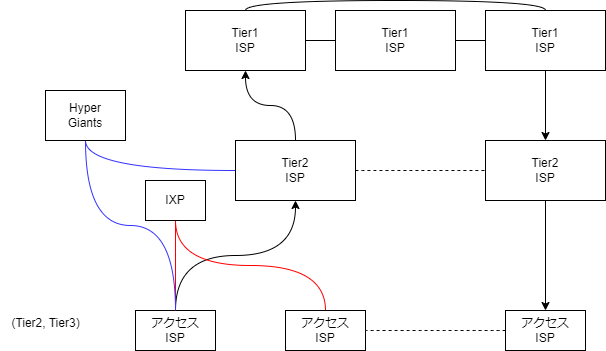
\includegraphics[width=0.6\linewidth]{image/isp.png}
  % \caption{}
  % \label{fig:}
\end{figure}

\newpage
\subsection{プロトコル階層とサービスモデル}

\subsubsection{階層化アーキテクチャ}

インターネットは極めて複雑なシステム
\begin{itemize}
  \item[] プロトコルならびに、それを動作させるハードウェア、ソフトウェアを階層化して設計
  \begin{itemize}
    \item[$\Rightarrow$] ネットワーク設計の複雑さを軽減し、各構成要素間の役割や関係を明確にする
    \item[] \textcolor{cyan}{モジュール化、個別に設計}
  \end{itemize}
\end{itemize}

各プロトコルはある一つの階層(layer)に属する
\begin{itemize}
  \item[] 第n層のプロトコルは第n層同士でメッセージを交換
  \begin{itemize}
    \item[] 第n層のプロトコルデータユニット(n-PDU): 第n層で交換されるメッセージ
  \end{itemize}
\end{itemize}

\begin{itemize}
  \item プロトコルスタック(protocol stack): これらのプロトコルが構成する階層全体
  \begin{itemize}
    \item[$\cdot$] OSI参照モデル(Open System Interconnection Refference Model): 7層構造
    \item[$\cdot$] インターネット(TCP/IP): 5層構造
  \end{itemize}
\end{itemize}

\begin{figure}[h]
  \centering
  
\includegraphics[width=0.8\linewidth]{image/npu.png}
\end{figure}


ホストAの第n層がホストBの第 n 層にn-PDUを送信
\begin{enumerate}
  \item ホストAの第n層がホストBの第 $n-1$ 層にn-PDUを渡し、ホストBの第n層への送信を依頼
  \item 第n層は第 $n-1$ 層のサービスを受ける  (第 $n-1$ 層は第n層にサービスを提供)
  \item 第n層は第 $n-1$ 層がどのようにサービスを実現しているかを意識しない
  \begin{itemize}
    \item[$\Rightarrow$] 層間のインターフェースが定義されていれば差し替え可能
    \item[] \textcolor{cyan}{抽象メソッドみたい}
  \end{itemize}
  \item[] \textcolor{cyan}{層が深くなるにつれ、誤り訂正などの処理が行われる}
\end{enumerate}


$\cdot$ プロトコル階層化の欠点
\begin{itemize}
  \item 同じ機能を複数の層が持つ場合がある (誤り制御など)
  \begin{itemize}
    \item[] \textcolor{cyan}{データ量的に無駄}
  \end{itemize}
  \item 上位層は下位層の情報を利用できない (柔軟性の欠如)
\end{itemize}


\newpage
\subsubsection{インターネットプロトコル階層}

\begin{table}[h]
  \centering
  \caption{}
  \label{tab:}
  \begin{tabular}{c|c|c}
    && PDUの呼び方\\\hline
    Layer 5 & アプリケーション & メッセージ \\
    Layer 4 & トランスポート & セグメント\\
    Layer 3 & ネットワーク データグラム(パケット)\\
    Layer 2 & データリンク & フレーム\\
    Layer 1 & 物理 & 1-PDU\\\hline
  \end{tabular}
\end{table}

\begin{itemize}
  \item アプリケーション層\\
    \underline{ネットワークアプリケーションをサポート}
  \begin{itemize}
    \item[例)] HTTP: web
    \item[] SMTP: 電子メール
    \item[] FTP: ファイル転送
  \end{itemize}
  \item トランスポート層\\
    \underline{アプリケーションプロセス間}のメッセージ転送サービスで提供
  \begin{itemize}
    \item TCP: 高信頼データ転送、フロー制御、輻輳制御
    \item UDP: コネクションレス型サービス
  \end{itemize}
  \item ネットワーク層\\
    始点・終点ホスト間でデータグラムの転送を行うIP・インターネットの3層プロトコル (IP層ともいう)
  \begin{itemize}
    \item[] IPデータグラムの定義と、それに基づくエンドシステムやルータの動作を規定
    \item ルーチングプロトコル:\\
      始点ホストから終点ホストまでの経路を設定\\
      複数のプロトコルが存在
    \end{itemize}
  \item データリンク層\\
    \underline{ノード間の1ホップ} の通信を担う
  \begin{itemize}
    \item[例)] Wi-Fi, イーサネット(有限LAN)など
  \end{itemize}
  \item 物理層
  \begin{itemize}
    \item フレーム内の各ビットを伝送
    \item \begin{tabbing}
      物理メディア: \=より対線、同軸ケーブル\\
      \>光ファイバ、無線など
    \end{tabbing}
  \end{itemize}
\end{itemize}

ネットワークエンティティ

\indent\indent ネットワークの構成要素(エンドシステムと中継器)
\begin{itemize}
  \item \begin{tabbing}
    中継器: \=ルータ(3層まで)\\
    \>ブリッジ、スイッチ(2層まで)
  \end{tabbing}
  \item エンドシステム: 5層すべて
\end{itemize}

\newpage
\section{アプリケーション層プロトコル}

\subsection{基礎}
\subsubsection{アプリケーション層プロトコル}

\begin{itemize}
  \item ネットワークアプリケーション: ネットワークの使用を前提とするソフトウェア
  \begin{itemize}
    \item[例)] Webアプリケーションは、ブラウザ(Chrome, Safariなど) とWebサーバ (Apacheなど) の複数のソフトウェアから構成
    \item[] \textcolor{cyan}{Webサーバは他にも nginxとか}
  \end{itemize}
\end{itemize}

\begin{itemize}
  \item アプリケーション層プロトコルは。メッセージ交換方法やメッセージのタイプ・フォーマットを規定
  \begin{itemize}
    \item[例)] webでは HTTP を使用
  \end{itemize}
  \item ネットワークアプリケーションは一般にクライアントとサーバの両方の側面をもつ (WebブラウザとWebサーバの関係)
  \item ネットワークを介した \textcolor{orange}{プロセス間通信}
  \item[] \textcolor{cyan}{プロセス間通信は実際には1つ下の層であるトランスポート層が提供 (自由度が高いらしい)}
  \begin{itemize}
    \item 二つのエンドシステムにあるプロセス間でネットワークを介してやり取り
    \item ソケット (Socket) と呼ばれる仮想的なインターフェースを用いる
    \begin{itemize}
      \item ソケットはAPI (Application Programming Interface) の一種
      \item トランスポート層とのインターフェースの役割
    \end{itemize}
  \end{itemize}
  % 黒板の改ページ
  \item コネクション (フロー) の単位
  \begin{itemize}
    \item[※] アプリケーション層が割り当てる情報
    \begin{itemize}
      \item 送受信ホストの \undercolor{IPアドレス}  % 1, 2
      \item プロセスの送受信 \undercolor{ポート番号} % 3, 4
      \begin{itemize}
        \item[$\rightarrow$] ホストのどのプロセスかを特定する番号
      \end{itemize}
      \item サーバ側プロセスは多くの場合ポート番号が固定
      \begin{itemize}
        \item 1023番まではwell-knownポートとして予約 (HTTP:80. SMTP:25, DNS:53 など)
      \end{itemize}
    \end{itemize}
  \end{itemize}
  \item トランスポート層プロトコル \undercolor{(TCP, UDP)}  % 5
  \item[] \textcolor{cyan}{同じポート番号でもプロトコルが違えば使用可能}
\end{itemize}
% 1,2,3,4,5 をまとめてなんか言ってた
% 5個情報送るよって話

\newpage
\subsubsection{トランスポート層プロトコルから提供されるサービス}

アプリケーション製作者は、「データ損失」「帯域幅」「遅延」の観点から選択

\begin{itemize}
  \item TCPサービス
  \begin{itemize}
    \item コネクション指向型: 全2重コネクション。ハンドシェイクを待ってから通信
    \item 高信頼データ伝送: 誤りのない、正しい順序のデータ送信を保証
    \item 輻輳制御: ネットワークの混雑に合わせて伝送レートを変更
  \end{itemize}
  \item UDPサービス
  \begin{itemize}
    \item 最小限のデータ伝送: メッセージの到達性や正確性は保証しない
    \item コネクションレス型: ハンドシェイクは行わない
    \item 輻輳制御なし: 伝送レートは始点プロセスで指定
  \end{itemize}
\end{itemize}

\subsubsection{アプリケーション層プロトコルの分類}

プル型、プッシュ型
\begin{itemize}
  \item プル型プロトコル
  \begin{itemize}
    \item HTTP, FTPなど
    \item ユーザが必要に応じて情報を引き出す (サーバが情報通信)
    \item 情報取得を希望するクライアントがコネクションを開始
    \end{itemize}
  \item プッシュ型プロトコル
  \begin{itemize}
    \item SMTPなど: (メールを送る側が相手へ情報送信)
    \item 情報発信する側がコネクションを開始
  \end{itemize}
\end{itemize}

個別帯域、共通帯域
\begin{itemize}
  \item 個別帯域 (out-of-band) 方式
  \begin{itemize}
    \item 制御用とデータ用で別のコネクションを使用\\
    \textcolor{cyan}{大きなファイルのアップロードの際に制御情報を別ルートで送ることができる}
    \item 代表例はFTP \textcolor{cyan}{Webページの更新など}
  \end{itemize}
  \item 共通帯域 (in-band 方式)
  \begin{itemize}
    \item 制御用とデータ用で同じコネクションを使用
      \textcolor{cyan}{(TCPを想定)}
    \item 代表例はHTTP
  \end{itemize}
\end{itemize}

個別帯域の例
\begin{itemize}
  \item 個別帯域の考え方は色々な場合に存在
  \item OpenFlow
  \item 5GのC/U 分離 (フェムトセル) \textcolor{cyan}{control, user \url{https://jirei.bzlog.jp/5g/information_14/}}
  \begin{itemize}
    \item マクロセルで制御信号をやり取り
    \item フェムトセルで高速データ転送
  \end{itemize}
\end{itemize}

\newpage
\subsection{WebとHTTP}
\subsubsection{HTTPの概要}

\begin{itemize}
  \item HTTP(Hypertext Transfer Protocol):\\
    Web用のアプリケーション層プロトコル
  \item Web ページ:\\
    基本となるHTMLファイルと、いくつかのWebオブジェクトの集合体\\
    URLにはホスト名やパス名、ファイル名が含まれる
  \item Webオブジェクト: HTMLファイル, 各種画像, JavaScript, 音声データ, 動画など
  \item Webブラウザ: Webページを表示するHTTPクライアント(Chrome, Safari, Edge, Firefox など)
  \item Webサーバ: Webオブジェクトを蓄えるHTTPサーバ(Apacheなど)
\end{itemize}

\begin{itemize}
  \item HTTPは、WebブラウザがWebサーバに対しWebページを要求する方法やサーバがそれに対して返送するための方法を定義
  \begin{itemize}
    \item 基本的に、クライアントがHTTP requestメッセージを送り、サーバがHTTP responseメッセージを返す % 板書だとresponce: たいぽ?
  \end{itemize}
  \item トランスポート層プロトコルはTCP\\
    (ソケットに渡したあとは到達性が保証される)
  \begin{enumerate}  % [(i), (ii), (iii), (iv)]
    \item クライアントがサーバのポート 80 へTCPコネクションを要求
    \item サーバとクライアントの間でTCPコネクションを確立
    \item HTTPメッセージをクライアント・サーバ間で交換
    \item TCPコネクションをクローズ
  \end{enumerate}
\end{itemize}

\begin{itemize}
  \item HTTPはステートレス(stateless)なプロトコル
  \begin{itemize}
    \item サーバはクライアントの履歴情報を記憶しない\\
      例えば同じクライアントから、同じ要求が2回届くとサーバは同じレスポンスを2回返す
    \item 制御が軽く、同時に多数のHTTP要求に対応可能\\
      状態を記憶する場合、状態の維持や故障・切断時の処理定義が別途必要
  \end{itemize}
  \textcolor{cyan}{ステートレス:履歴をもたない (一昔前のチャットボットみたいな感じ?)}\\
  \textcolor{cyan}{webの情報はクライアント側が保持(cookie?)}
\end{itemize}

\subsubsection{非継続型コネクションと継続型コネクション}

\begin{itemize}
  \item 非継続型コネクション( non-persistent connection)
  \begin{itemize}
    \item 一つのTCPコネクションは一つのWebオブジェクトを転送
    \item 通常ブラウザは並列して5から10のTCPコネクションをはれるが埋まっていれば、各オブジェクトは直列に処理される
    \item HTTP/1.0で使用
  \end{itemize}

  \begin{itemize}
    \item 非継続型の欠点
    \begin{itemize}
      \item 多くのTCPコネクションをサーバが管理する必要
      \item 各オブジェクトの転送に、2RTT必要(TCPコネクションの確立に1RTT要する)
      \item[] ※ RTT(Round Trip Time: 往復遅延時間)
    \end{itemize}
  \end{itemize}
\end{itemize}

\begin{itemize}
  \item 継続型コネクション(Persistent connection)
  \begin{itemize}
    \item 一つのコネクションで複数のWebオブジェクトを転送
    \item サーバは応答を返した後もTCPコネクションを継続
    サーバで認定された一定時間(タイムアウト時間)使用されたなければコネクションを切断
    HTTP/1.1 のデフォルト
  \end{itemize}
\end{itemize}

パイプライン処理
\begin{itemize}
  \item 非パイプライン処理型 (without pipelinig)
  \begin{itemize}
    \item クライアントは応答メッセージの受信を待ってから、次の要求メッセージを送信
  \end{itemize}
  \item パイプライン処理型 (with pipelinig)
  \begin{itemize}
    \item クライアントは応答メッセージを受け取るまえに、次々と要求メッセージを送信可能
  \end{itemize}
\end{itemize}

\subsubsection{HTTPメッセージ}

\begin{itemize}
  \item 2種類のメッセージ: リクエスト(要求), レスポンス(応答)
  \item HTTPリクエストメッセージ
  \begin{itemize}
    \item \begin{tabbing}
      リクエスト行: \=HTTPメソッド(GET, POSTなど)\\
      \>リクエスト対象(URL) \\
      \>HTTPバージョン
    \end{tabbing}
    \item ヘッダ行   : user agent などを key:value形式でストア
    \item 本文
  \end{itemize}
  \item HTTP応答メッセージ
  \begin{itemize}
    \item \begin{tabbing}
      ステータス行: \=ステータスコード(200, 403, 404, 503など)\\
      \> ステータス文字列(OK, Permission Denied, Not Found, Service Unavailable など)
    \end{tabbing}
    \item ヘッダ行: ViaやContent-lengthなどを key:value形式でストア
    \item 本文
  \end{itemize}
\end{itemize}

\newpage
\subsubsection{HTTP/2}

2015年5月にRFC文書化された新しいHTTPのバージョン (5年ぶりのアップデート)

\begin{itemize}
  \item \begin{tabbing}ストリ\=ーム: \=コネクション上にレスポンスとリクエストが多重化された仮想的な双方向シーケンス\\
      \>ストリームの多重化により、オブジェクトの同時送受信が可能\\
      \>\>\textcolor{orange}{$\rightarrow$ HoL (Head of Line) ブロッキング} \footnotemark の解消\\  %ホルブロッキング
    \>(例えば Apache では、100ストリームの多重化が可能)
  \end{tabbing}\footnotetext{
        HoLブロッキング問題: レスポンスにおいて、リクエストの順に返す必要があるため、大きなオブジェクトの伝送が詰まると待ち時間が発生してしまう
      }
    % ※HoLブロッキング問題: レスポンスにおいて、リクエストの順に返す必要があるため、大きなオブジェクトの伝送が詰まると待ち時間が発生してしまう
  \item HPACkによるHTTPヘッダの圧縮 (二回目以降は差分で通信)\\
  \textcolor{cyan}{サーバなど大規模なものであればヘッダの圧縮の効果が大きい}
  \begin{itemize}
    \item[※] HTTP/1.1ではコンテンツのみ.gz圧縮
  \end{itemize}
  \item HTTP/2フレーム: フレームという形式のバイナリデータによる通信(これまでは全てテキストベース)
  \begin{itemize}
    \item HTTPヘッダとデータをそれぞれフレーム単位で分割(ヘッダ圧縮にも対応)
    \item フレーム分割や圧縮は HTTP/1.X のメッセージに対し透過的(HTTPの下層に配置。アプリケーションの製作者は通常どおりにHTTPを利用すればよい)\\
    \textcolor{cyan}{アプリケーション層とトランスポート層の間で動作。アプリケーション層では通常のHTTPとして処理されるため、HTTP/1.1でも動作する}
  \end{itemize}
  \item サーバプッシュ(レスポンスに必要なデータを事前にサーバからクライアントへ送信)\\
  \textcolor{cyan}{GETリクエストが来た際に必要そうなものを予め送信}
  \item ストリームの優先制御
  \item HTTP/2は、ほとんどの主要ブラウザがサポート\\
  \textcolor{cyan}{10年前の技術であるためサポートされているが、そこまで早くする必要性がない場合もありHTTP/1も現役}
  \item TCP以外でも動作を想定
\end{itemize}

\newpage
\subsubsection{HTTPストリーミングとDASH}

\begin{tabbing}
  DASH\= (Dynamic Adaptive Streaming over HTTP)\\
  \>※正式にはMPEGDASH
\end{tabbing}

\begin{itemize}
  \item 動画ファイルを異なるビットレートを持つ複数のバージョンにエンコード(圧縮)\\
    \textcolor{cyan}{動画の場合は画像毎の差分をとったりして圧縮}
  \item セグメントに分割され、サーバ側で保持(数秒から数十秒単位)
  \item クライアントは、帯域に応じて、\textcolor{cyan}{(動的に)} 適切な圧縮率のセグメントをリクエスト\\
    (混んでいるときは、低品質を選ぶ)
  \item HTTPサーバはMPD (Media Presentation Description)保持 \textcolor{cyan}{(MPDという設定ファイル)}
  \begin{itemize}
    \item 各バージョンのセグメントのURLを記載
    \item クライアントは、最初にMPDをリクエスト
  \end{itemize}
  \item 各セグメントの取得は、通常のHTTP GET でリクエスト
  \item \textcolor{cyan}{appleはMPEG DASHには対応せずHLSという別の規格が存在\\
    \url{https://www.cloudflare.com/ja-jp/learning/video/what-is-mpeg-dash/}
  }
\end{itemize}


\subsection{FTP}

\begin{itemize}
  \item 個別帯域(out-of-band)方式のプロトコル
  \item データ転送に利用
  \item 二つのコネクションを利用
  \begin{itemize}
    \item 制御コネクション: ポート21、継続型
    \begin{itemize}
      \item ユーザ認証、cd、put、getなどのコマンド
    \end{itemize}
    \item データコネクション: ポート20、非継続型
    \begin{itemize}
      \item 実際のファイル転送を担う
      \item \textcolor{cyan}{1ファイルずつ、必要に応じて}
    \end{itemize}
  \end{itemize}
\end{itemize}

\newpage
\subsection{電子メール}

構成要素
\begin{itemize}
  \item ユーザエージェント (メーラ)  % thunder birdとか
  \item メールサーバ (postfixなど)
  \item \begin{tabbing}
    プロトコル: \=SMTP(Simple Mail Transfer Protocol)\\
    \>メールアクセスプロトコル
  \end{tabbing}
  \item 始点エージェントサーバ間およびサーバ間の通信はSMTPを使用
  \item メールサーバ終点エージェント間はメールアクセスプロトコルを使用
  \begin{itemize}
    \item POP3 (Post Office Protocol ver.3)
    \item IMAP (Internet Mail Access Protocol)
  \end{itemize}
\end{itemize}

\subsubsection{SMTP}

\begin{itemize}
  \item 始点側メールサーバ (クライアント) から終点側メールサーバへのメッセージ転送
  \item データ形式は7ビットASCIIコード
  \begin{enumerate}
    \item クライアントはサーバにポート25番でTCP接続
    \item アプリケーション層でハンドシェイク
    \begin{enumerate}
      \item クライアントが送信元アドレスを知らせ、サーバ送信許可を返す
      \item クライアントは宛先アドレスをサーバへ知らせ、サーバは、宛先アカウントの有無をクライアントに通知
    \end{enumerate}
    \item クライアントはデータ送信開始を通知し、サーバの返答を受け取ると送信開始
    \item 送信終了後、TCPコネクションを切断
  \end{enumerate}
  \item TCPコネクションは継続型
  \begin{itemize}
    \item[] 同じサーバ宛のメールが複数あれば、同じコネクションを使って送信可能
  \end{itemize}
\end{itemize}


\newpage
\subsection{DNS (Domain Name System)}

\begin{itemize}
  \item ネームサーバによる階層的データベース
  \item ホストとネームサーバ間の通信を担うアプリケーション層プロトコル
\end{itemize}

\subsubsection{提供されるサービス}

\begin{itemize}
  \item ホスト名をIPアドレスに変換 (\textbf{名前決定})
  \item ホスト名の別名 (alias: エイリアス) の登録
  \item メールサーバ名の別名登録
\end{itemize}

\begin{itemize}
  \item DNSラウンドロビン: 負荷分散
  \begin{itemize}
    \item 公式ホスト名と複数のミラーサーバのIPアドレスの集合を対応づけ問い合わせ毎にIPアドレスをシフトして通知\\
      (クライアントはリストの一番上を使う)
  \end{itemize}
\end{itemize}

\subsubsection{DNSの仕組み}

\begin{itemize}
  \item \textbf{なぜ集中型でないか}
  \item 分散型モデル(ネームサーバの分類)
  \begin{itemize}
    \item 障害発生時の信頼性欠如(single point of failure)
    \item サーバへのトラヒック集中
    \item 遠隔地との通信遅延が大きい
    \item 保守更新の煩雑さ
  \end{itemize}
  \item 分散型モデル(ネームサーバの分類)
  \begin{itemize}
    \item ルートDNSサーバ(世界で13系統)
    \begin{itemize}
      \item トップレベルDNSサーバのIPアドレスを把握
    \end{itemize}
    \item トップレベルドメイン(top-level domain)DNSサーバ
    \begin{itemize}
      \item jp, com, eduなどのトップレベルドメインを管理
    \end{itemize}
    \item 権威(Authoritative)DNSサーバ
    \begin{itemize}
      \item ホスト名(ドメイン名)とIPアドレスの変換機能を持つ
      \item 各ホストは必ず一つ以上の権威DNSサーバに登録
    \end{itemize}
    \item[※] ローカルDNSサーバ:DNSキャッシュサーバ、DNSリゾルバ
    \begin{itemize}
      \item ISPや各企業が個別に持つ
      \item ユーザは通常、ローカルDNSサーバに名前解決を依頼
    \end{itemize}
  \end{itemize}
  \item DNS反復クエリとDNS再帰クエリ
  \begin{itemize}
    \item DNS反復クエリ
    \begin{itemize}
      \item 問い合わせたネームサーバへの名前の解決を依頼
    \end{itemize}
    \item DNS再帰クエリ
    \begin{itemize}
      \item 問い合わせるべきネームサーバの情報を要求
    \end{itemize}
  \end{itemize}
\end{itemize}

\begin{itemize}
  \item ローカルDNSサーバはホストへ転送した情報をキャッシュする:DNSキャッシュ
  \item DNSレコード
  \begin{itemize}
    \item リソースレコードを格納する分散データベース
    \item (name, value, type, ttl)の4フィールドで構成
    \item Type A レコード
    \begin{itemize}
      \item nameはホスト名, valueはIPadoresu (IPv6の場合、AAAAレコード)
    \end{itemize}
    \item Type NS レコード
    \begin{itemize}
      \item nameはドメイン名, valueはその権威DNSサーバホスト名
    \end{itemize}
    \item Type CNAMEレ コード
    \begin{itemize}
      \item ホスト名の別名
    \end{itemize}
    \item Type MX レコード
    \begin{itemize}
      \item nameに関するメルサーバ情報を格納
    \end{itemize}
  \end{itemize}
  \item TTLは秒単位で記載
  \begin{itemize}
    \item この期間を過ぎるとキャッシュから削除
  \end{itemize}
\end{itemize}

\subsubsection{DNSサーバへの攻撃}
\begin{itemize}
  \item DNSキャッシュポイズニング
  \begin{enumerate}
    \item 攻撃者がDNSキャッシュサーバへ名前解決を依頼
    \item DNSキャッシュサーバは再帰的に問合せ
    \item 攻撃者は即座に、偽装したUDPパケットで返答
    \item キャッシュサーバは、誤ったドメイン情報を記憶
  \end{enumerate}
  \item[※] 攻撃要件
  \begin{enumerate}
    \item 発信元DNSサーバのIPアドレスに偽装
    \item 問い合わせと同じUDPポート番号を使用
    \item 問い合わせと同じID(6/bit)を使用
    \item 本来のDNSサーバより先に応答
    \begin{itemize}
      \item さらに、攻撃のチャンスはTTL毎に一度だけ
    \end{itemize}
  \end{enumerate}
\end{itemize}

\newpage
\subsection{コンテンツ分散}

\begin{itemize}
  \item コンテンツが一つのサーバ上のみにあると
  \begin{itemize}
    \item 伝送遅延が増大
    \item サーバへの負担が大きい
  \end{itemize}
  \item コンテンツ分散
  \begin{itemize}
    \item コンテンツをインターネット上の複数サーバにコピー
    \item ユーザに最も迅速に配送できるサーバを見つけ、コンテンツを配信
  \end{itemize}
\end{itemize}

\subsubsection{CDN (Content Distribution Network)}
\begin{itemize}
  \item 90年代後半から登場したビジネスモデル
  \item CDNサービス企業は、インターネット上に多数のサーバ(CDNサーバ)を配置
  \begin{itemize}
    \item (NetfrixやYoutubeは自社でCDNサーバを設置)
    \item 顧客のコンテンツをCDNサーバにコピー(各更新毎に)
    \item ユーザのコンテンツを要求に対して、適切なCDNサーバを選択
  \end{itemize}
  \item[$\rightarrow$] \textbf{ユーザごとにDNSの返答を変える}
\end{itemize}

\newpage
\section{トランスポート層}

\subsection{トランスポート層サービス}

アプリケーションプロセスへ、通信サービスを直接提供
\begin{itemize}
  \item アプリケーションを実行するエンドシステムに組み込まれている
  \item ネットワーク内のルータには通常組み込まれない
\end{itemize}

\undercolor{アプリケーションプロセス}間に、\undercolor{論理的通信路}を提供
\begin{itemize}
  \item アプリケーションは、物理的通信インフラの構造を意識しない
\end{itemize}


\subsubsection{トランスポート層とネットワーク層の関係}

ネットワーク層: \undercolor{ホスト間}の\undercolor{論理的通信路}を提供
\begin{itemize}
  \item[] インターネット (IP) では、\undercolor[black]{ベストエフォート}
  \footnote{何も保証しない}
  型転送サービス
\end{itemize}
アプリケーションから見たとき、トランスポート層がないと、
\begin{itemize}
  \item アプリケーション固有の要求に応じた適切な通信サービスが受けられない
  \item 物理的特性あるいはネットワークの輻輳により、通信インフラの信頼性が低い場合に対処できない
\end{itemize}

% メモリ上に展開されてプロセスとなる、トランスポート層はプロセス間の通信を担う
% ネットワーク層は基本的には端末から端末への通信を担う


\subsubsection{インターネットのトランスポート層}

最小限度の機能 (UDP, TCPともに備える)
\begin{itemize}
  \item プロセス間の転送サービス
  \item \undercolor[black]{セグメント}\footnote{
      トランスポート層PDU
    }の伝送誤り検査
\end{itemize}

UDP (User Datagram Protocol): 信頼性を保証しないコネクションレス型サービス
\begin{itemize}
  \item[] 最小限度の機能のみを持つ
\end{itemize}

TCP (Transmission Control Protocol): 信頼性の高い、コネクション指向型サービス
\begin{itemize}
  \item[] 最小限度の機能に加えて
  \begin{itemize}
    \item 誤りのない、正しい順序でのセグメント転送を保証
    \item 輻輳制御とフロー制御による、送信レート制御を提供
  \end{itemize}
\end{itemize}


\newpage
\subsection{多重化と逆多重化}
% 一旦文字列の幅を確認したいから、ここに内容はないけどやや長めの文章を書いていこうと思う。お気持ち的な文章は内容の割に長さを稼げるように思う
\begin{tabbing}
  タブ調整用の文字列、これは\=表示されない \kill
  \measuretab{タブ調整用の文字列、これは}
  % 多重化 (multiplexing): \>様々なソケット (アプリケーションとのインターフェース) からトランスポート層\\\>へ送出されたセグメントをまとめてネットワーク層へ引き渡す\\
  多重化 (multiplexing): \>\wraptab{様々なソケット (アプリケーションとのインターフェース) からトランスポート層へ送出されたセグメントをまとめてネットワーク層へ引き渡す}\\

  逆多重化 (demultiplexing): \>ネットワーク層から取り出されたセグメントを適切なソケットへ渡す
\end{tabbing}

ポート番号: ソケットを識別する番号 (0から 65535 ($2^{16}-1$))
\begin{itemize}
  \item 0 から 1023 までは well-known ポート番号として予約
  \item TCP と UDP で区別 (両者で同じ番号が使える)
\end{itemize}

クライアントがUDPあるいはTCPソケットを作り、ポート番号を付加\\
\indent(通常は 1024 番号以降からランダムに選択)

サーバ側では well-known ポート番号を使用


\subsubsection{UDP}

% クライアント: 始点ポート番号と終点ポート番号をヘッダに付加し、(ソケットへbindし)多重化

% サーバ: 終点ポート番号 (とIPアドレス) のみに基づいてソケットを選択

%         (異なるクライアントからのセグメントでも同じソケットへ渡される)
%         始点ポート番号は、返信の際の終点ポート番号として使用
\begin{tabbing}

クライアント: \=始点ポート番号と終点ポート番号をヘッダに付加し、(ソケットへbindし)多重化\\
サーバ: \>終点ポート番号 (とIPアドレス) のみに基づいてソケットを選択\\
        \>(異なるクライアントからのセグメントでも同じソケットへ渡される)\\
        \>始点ポート番号は、返信の際の終点ポート番号として使用
\end{tabbing}



\subsubsection{TCP}

クライアント: UDPと同じ

サーバ: 始点IPアドレス、始点ポート番号、終点IPアドレス、終点ポート番号でソケットを選択


\subsection{UDP}

\begin{itemize}
  \item 8バイトのヘッダ + ペイロード ( = アプリケーション層メッセージ)
  % figure 中央16bitずつ
  % |<----------32  bit---------->|
  % | 始点ポート番号| 終点ポート番号|
  % |セグメントの長さ|チェックサム  |
  % | アプリケーション層メッセージ  |

  \begin{table}[htbp]
  \centering
  \begin{tikzpicture}
      % 縦線
      \draw (0,2.5) -- (0,3.2);
      \draw (6,2.5) -- (6,3.2);

      % 32ビット矢印と表示
      \draw[<-] (0,2.85) -- (2.2,2.85);
      \node at (3,2.85) {32ビット};
      \draw[->] (3.8,2.85) -- (6,2.85);

      % 表の枠線
      \draw (0,2.5) -- (6,2.5);
      \draw (0,1.83) -- (6,1.83);
      \draw (0,1.17) -- (6,1.17);
      \draw (0,0) -- (6,0);
      \draw (0,0) -- (0,2.5);
      \draw (6,0) -- (6,2.5);
      \draw (3,2.5) -- (3,1.17);

      % テキスト
      \node at (1.5,2.17) {始点ポート番号};
      \node at (4.5,2.17) {終点ポート番号};
      \node at (1.5,1.5) {セグメントの長さ};
      \node at (4.5,1.5) {チェックサム};
      \node[above] at (3,0.58) {アプリケーション層メッセージ};
    \end{tikzpicture}
\end{table}


  \item 受信側でチェックサムを用いて誤り検出を行う
  \begin{itemize}
    \item[] チェックサム: 16ビット語を全て足したものの1の補数
  \end{itemize}
  \item これ以外は何もせず、必要最低限のトランスポート層サービスを提供
  \begin{itemize}
    \item メッセージを直接IP層へ渡す
  \end{itemize}
  \item[] 使用例: DNS, SNMPなど
\end{itemize}

\begin{itemize}
  \item \undercolor[black]{UDPを用いる利点}
  \begin{enumerate}
    \item 送るべきデータとその送出タイミングをアプリケーションから制御可能
    \begin{itemize}
      \item TCPの制約から解放、高信頼データ転送は、必要に応じてアプリケーション側で実装
    \end{itemize}
    \item コネクションの確立が不要: 遅延の減少
    \item コネクションの管理が不要
    \begin{itemize}
      \item[] サーバでのオーバヘッドが小さく、多くのクライアントと通信可能
    \end{itemize}
    \item ヘッダが小さく、伝送効率が高い (UDP 8バイト, TCP 20バイト)
  \end{enumerate}
\end{itemize}
% tcp -> udpの順にできた

\newpage
\subsection{高信頼データ転送}

高信頼データ転送(reliable data transmission)
\begin{itemize}
  \item 誤り (0, 1の反転) がなく、かつ、送信された順序通りに届く
  \item エンド-エンドの制御でどうやって実現するのか
  \begin{itemize}
    \item[$\Rightarrow$] \textcolor{orange}{ARQ (Automatic Repeat reQuest)} プロトコルによる制御
    \item 誤り検知・送達確認を行いながら、必要に応じて再送
  \end{itemize}
\end{itemize}

% 高信頼データ転送に必要なもの

\vskip\baselineskip
\noindent シナリオ1. パケットが壊れる (ビットエラーが発生する) 通信路

誤り検知と送達確認
\begin{itemize}
  \item ACK (Acknowledgement): 正しく受信されたことを伝える
  \item NACK (NegativeACK): 正しく受信されなかったことを伝える
\end{itemize}

\undercolor[black]{ストップアンドウェイト(SW: Stop and Weit)} プロトコル
\begin{itemize}
  \item パケットは一つずつ送信 (受信バッファサイズ1)
  \item ACK/NACK を受け取ったら、次のパケットを送信
  \begin{itemize}
    \item NACKの場合、再送
  \end{itemize}
\end{itemize}

\vskip\baselineskip
\noindent シナリオ1.1 ACK/NACK も壊れる場合

\begin{itemize}
  \item ACK/NACK が壊れると、正しく受け取れたか判断できない
  \item ACK を再送したとしても、それが「どのパケットのACKか」がわからない
  \item[$\Rightarrow$] パケットに \textcolor{orange}{シーケンス番号} を付与
  \begin{itemize}
    \item SWの場合、1ビットで十分
    \item[$\rightarrow$] 再送中であるかを表すフラグ
  \end{itemize}
\end{itemize}

\vskip\baselineskip
\noindent シナリオ1.1': 1.1 と同様の状況で、NACKを使用しない

同じシーケンス番号のACKが2度届けば、NACKと同じ効果

\textcolor{cyan}{1,0が交互にくるはずだから、連続で同じ数値の場合は再送とわかる}

\vskip\baselineskip
\noindent シナリオ 2.0; パケットロスが発生する通信路

パケットがそもそも到着しないので、エラーが検知できない
\begin{itemize}
  \item[$\Rightarrow$] \textcolor{orange}{タイムアウト時間} を設定
  \begin{itemize}
    \item タイムアウト時間内にACKを受信したら、次のパケットを送信
    \item タイムアウト時間内にACKを受信しなければ、再送
  \end{itemize}
  \item[※] 遅延 $>$ タイムアウト時間のとき、ロスがないのに再送してしまう
\end{itemize}

\subsubsection{ストップアンドウェイト(SW)}

\begin{itemize}
  \item 送信側
  \begin{itemize}
    \item パケットにシーケンス番号を付加 (1bit)
    \item タイムアウト時間を設定 (通常、 RTTより大きくとる)
    \textcolor{cyan}{RTT: 往復遅延時間 \ref{rtt_ref}参照}
  \end{itemize}
  \begin{enumerate}
    \item 次に送るべきパケット (番号順) を送信
    \item ACKの受信を待つ
    \begin{enumerate}
      \item タイムアウト時間内にACKを受信したら 1 へ
      \item タイムアウト時間内にACKを受信しなければ送信を失敗したものとみなし、 1 へ
    \end{enumerate}
  \end{enumerate}
  \item 受信側
  \begin{enumerate}
    \item パケットを受け取ったら、誤りがないか確認
    \item 誤りがなければ、そのパケットのシーケンス番号を付加したACKを返信
  \end{enumerate}
\end{itemize}

\begin{figure}[h]
% workflow
% こういった図は送信側・受信側それぞれで考える必要がある、らしい
% 受信側: ちゃんと届いたもののシーケンス番号を付加したACKを返すだけ
% 送信側: ACKが返ってきたら次のデータを送信するだけ
  \centering
  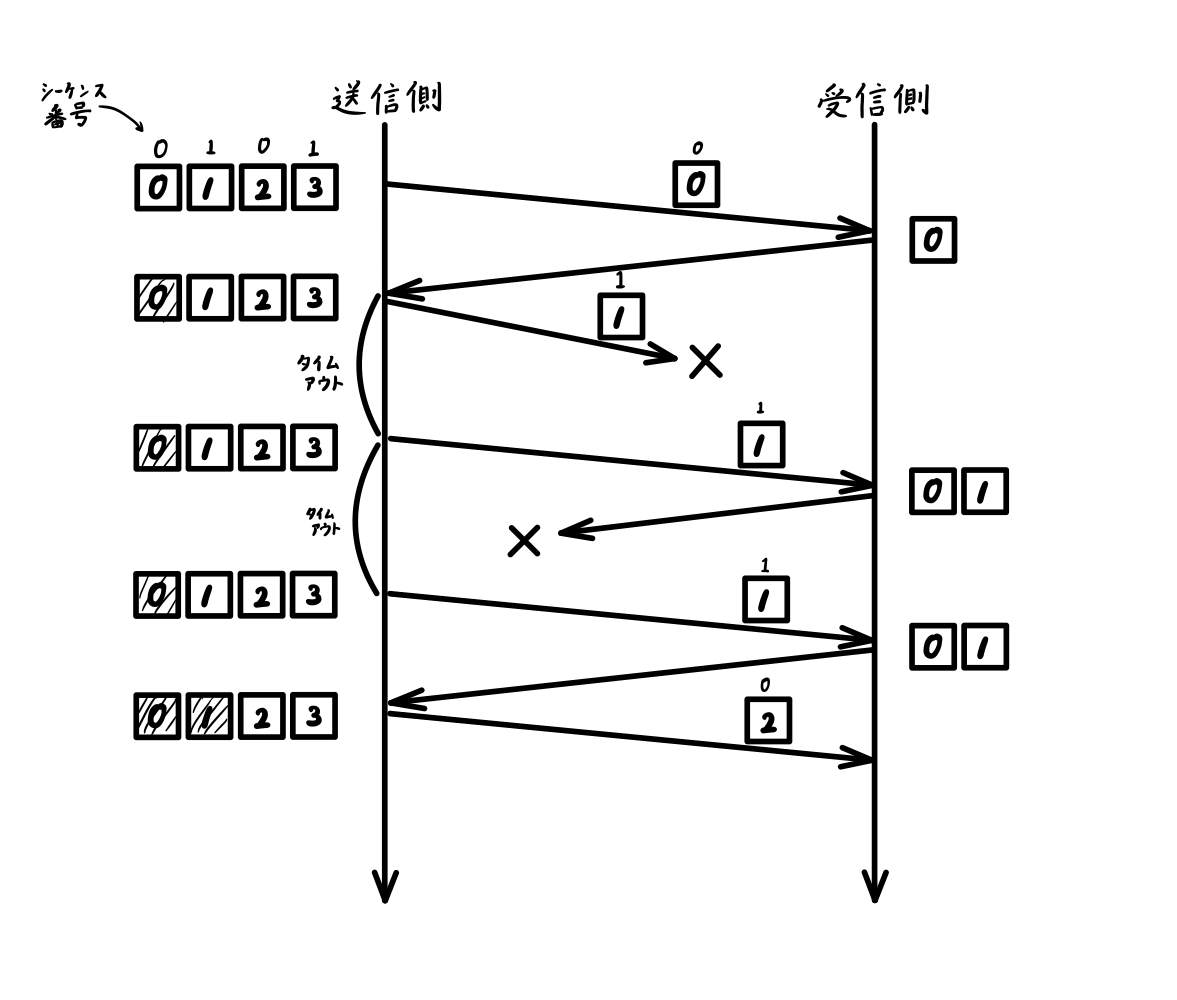
\includegraphics[width=0.65\linewidth]{image/stop_and_wait.png}
\end{figure}

\begin{itemize}
  \item SWの性能の概算
  \begin{itemize}
    \item データパケット長 $L$(bit), 回線速度 $R$ (bit/S), 往復遅延時間 $RTT$ (s)
    \item 1パケットの伝送にかかる時間 $RTT + \frac{L}{R}$
    \begin{itemize}
      \item スループット $\theta = \frac{L}{RTT+\frac{L}{R}}$
      \item 回線利用率 $U = \frac{\theta}{R} = \frac{L}{R \times RTT + L}$
      \item $R\times RTT$: \textcolor{orange}{帯域遅延積(Bandwidth-Delay Product)}
      \item 帯域遅延積が大きくなると回線利用率が低下
      \item[$\rightarrow$] 性能劣化の原因はACK待ちに要する時間
      \item[] \undercolor[black]{パイプライン化}により、性能は向上
    \end{itemize}
  \end{itemize}
\end{itemize}
% SWは大量のデータを流せる回線で使用すると非効率 時間的分割・ラウンドロビンとかRTOSとかに近い感じ?


\subsubsection{Go-back-N (GBN)}

\begin{itemize}
  \item ACKの受信を待たずに、連続するパケットを最大N個まで送信\\
    (スライディングウィンドウプロトコル)
  \item 送信失敗を確認すると、そのパケットから全てやり直し
  \begin{itemize}
    \item 受信した順序が入れ替わっていたら、パケットを捨てる\\
      \textcolor{cyan}{ACKが来ないとウィンドウが進めなくなる}
  \end{itemize}
\end{itemize}
\textcolor{cyan}{受信側が簡単な仕様、TCPはざっくりGo-back-Nだけど、すぐに捨てるわけじゃないみたい}

\begin{figure}[h]
% img 0~6の情報を3つずつ送信してる図
  \centering
  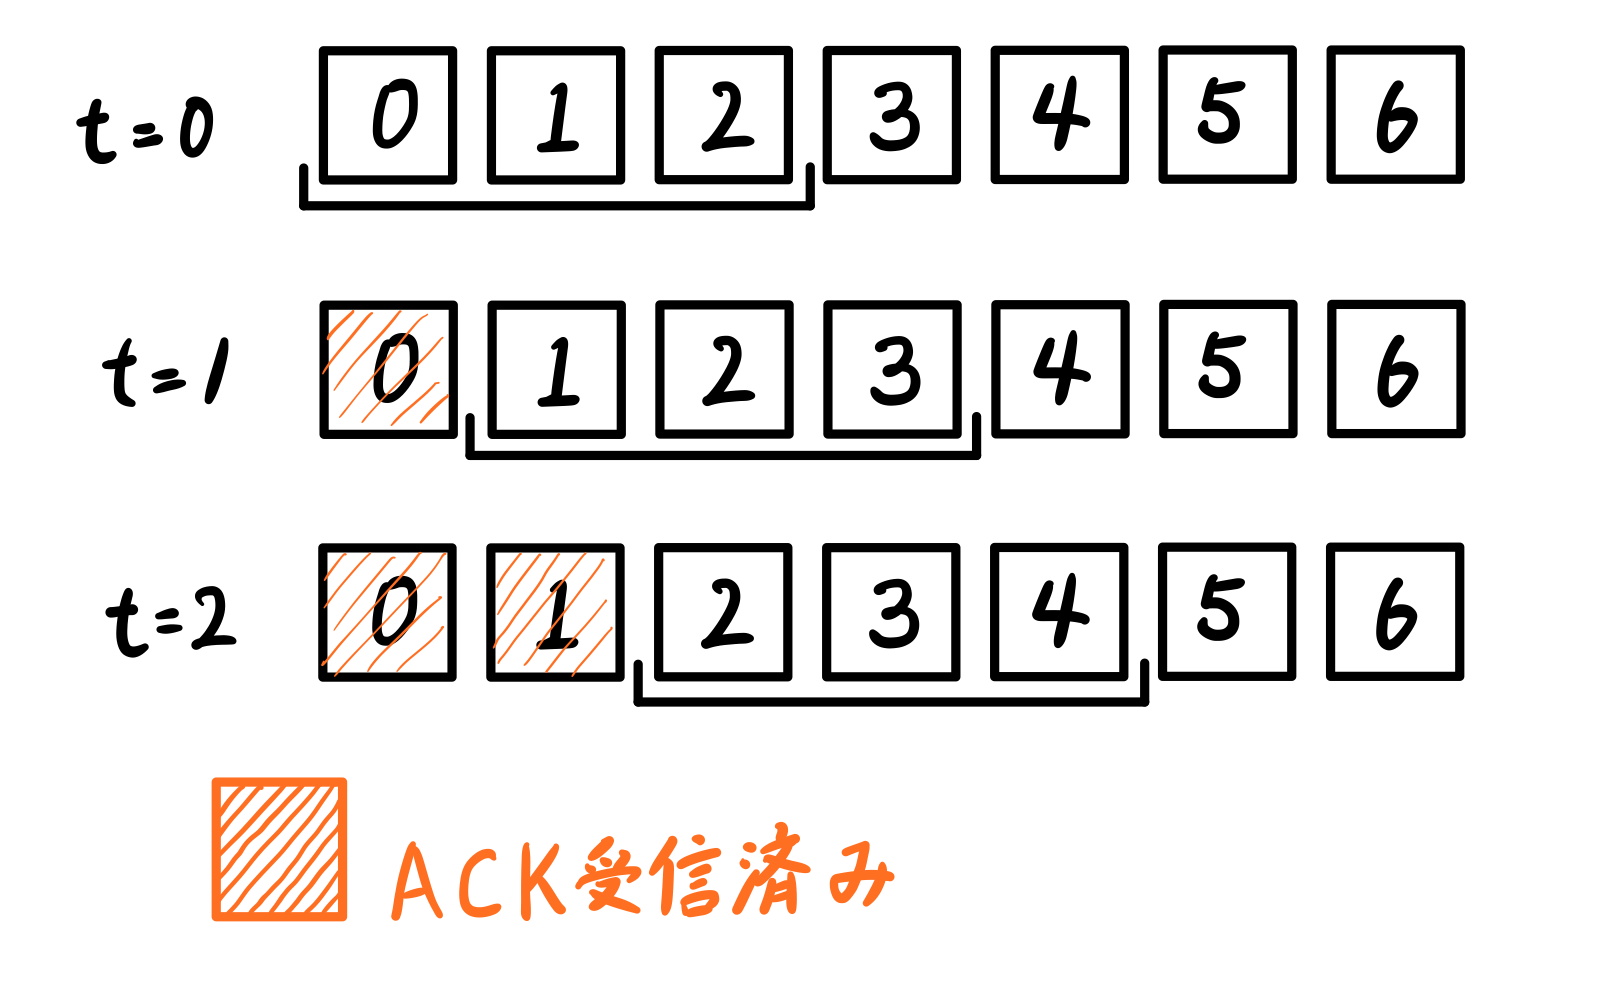
\includegraphics[width=0.4\linewidth]{image/go_back_n.png}
\end{figure}

\newpage
\subsubsection{GBN (Go-back-N)}

\begin{itemize}
  \item ACKの受信を待たずに、連続するパケットを最大N個まで送信可 (スライディングウィンドウ方式)
  \item 送信失敗が確認されると、そのパケットからやり直し(受信側のバッファサイズは 1)
\end{itemize}
\begin{itemize}
  \item 送信側\\
    パケットにシーケンス番号を付加  ($k$ビット)\\
    ウィンドウサイズ N(N$ < 2^k$)とタイムアウト時間を設定
  \begin{itemize}
    \item F: 送信したが、ACK未受信のパケット数
  \end{itemize}
  \begin{enumerate}
    \item 次に送るべきパケット(番号順)を F$=$N になるまで連続して送信
    \item 各パケットに対するACKを待つ
    \begin{enumerate}
      \item タイムアウト時間までにACKを受信したら、1へ
      \item タイムアウト時間までにACKを受信しなければ以降のパケットを受信失敗とみなして、1へ
    \end{enumerate}
  \end{enumerate}
  \item 受信側
  \begin{enumerate}
    \item パケットを受け取ったら、誤りがなく、正しい順序のパケットか確認
    \item 誤りがなく、正しい順序ならば、そのシーケンス番号を付加したACKを送信
    \item そうでなければ、そのパケットを破棄し、正しい順序で受け取った最後のパケットのシーケンス番号を付加したACKを送信
  \end{enumerate}
\end{itemize}

\vskip\baselineskip
\textcolor{orange}{累積ACK (Cumulative ACK)}
\begin{itemize}
  \item 付加されたシーケンス番号以前のパケットが全て正しく受信されたことを示す
  (ACKを一つにまとめる)
\end{itemize}

\begin{figure}[h]
% img: 左側はACKの失敗なし、右側は再送あり
% ウィンドウサイズ分をまとめて送信

% 一番都合の悪い場合
% 0 から 3 のパケットを受信成功したが、それに対するACKが全てロスした場合
  \centering
  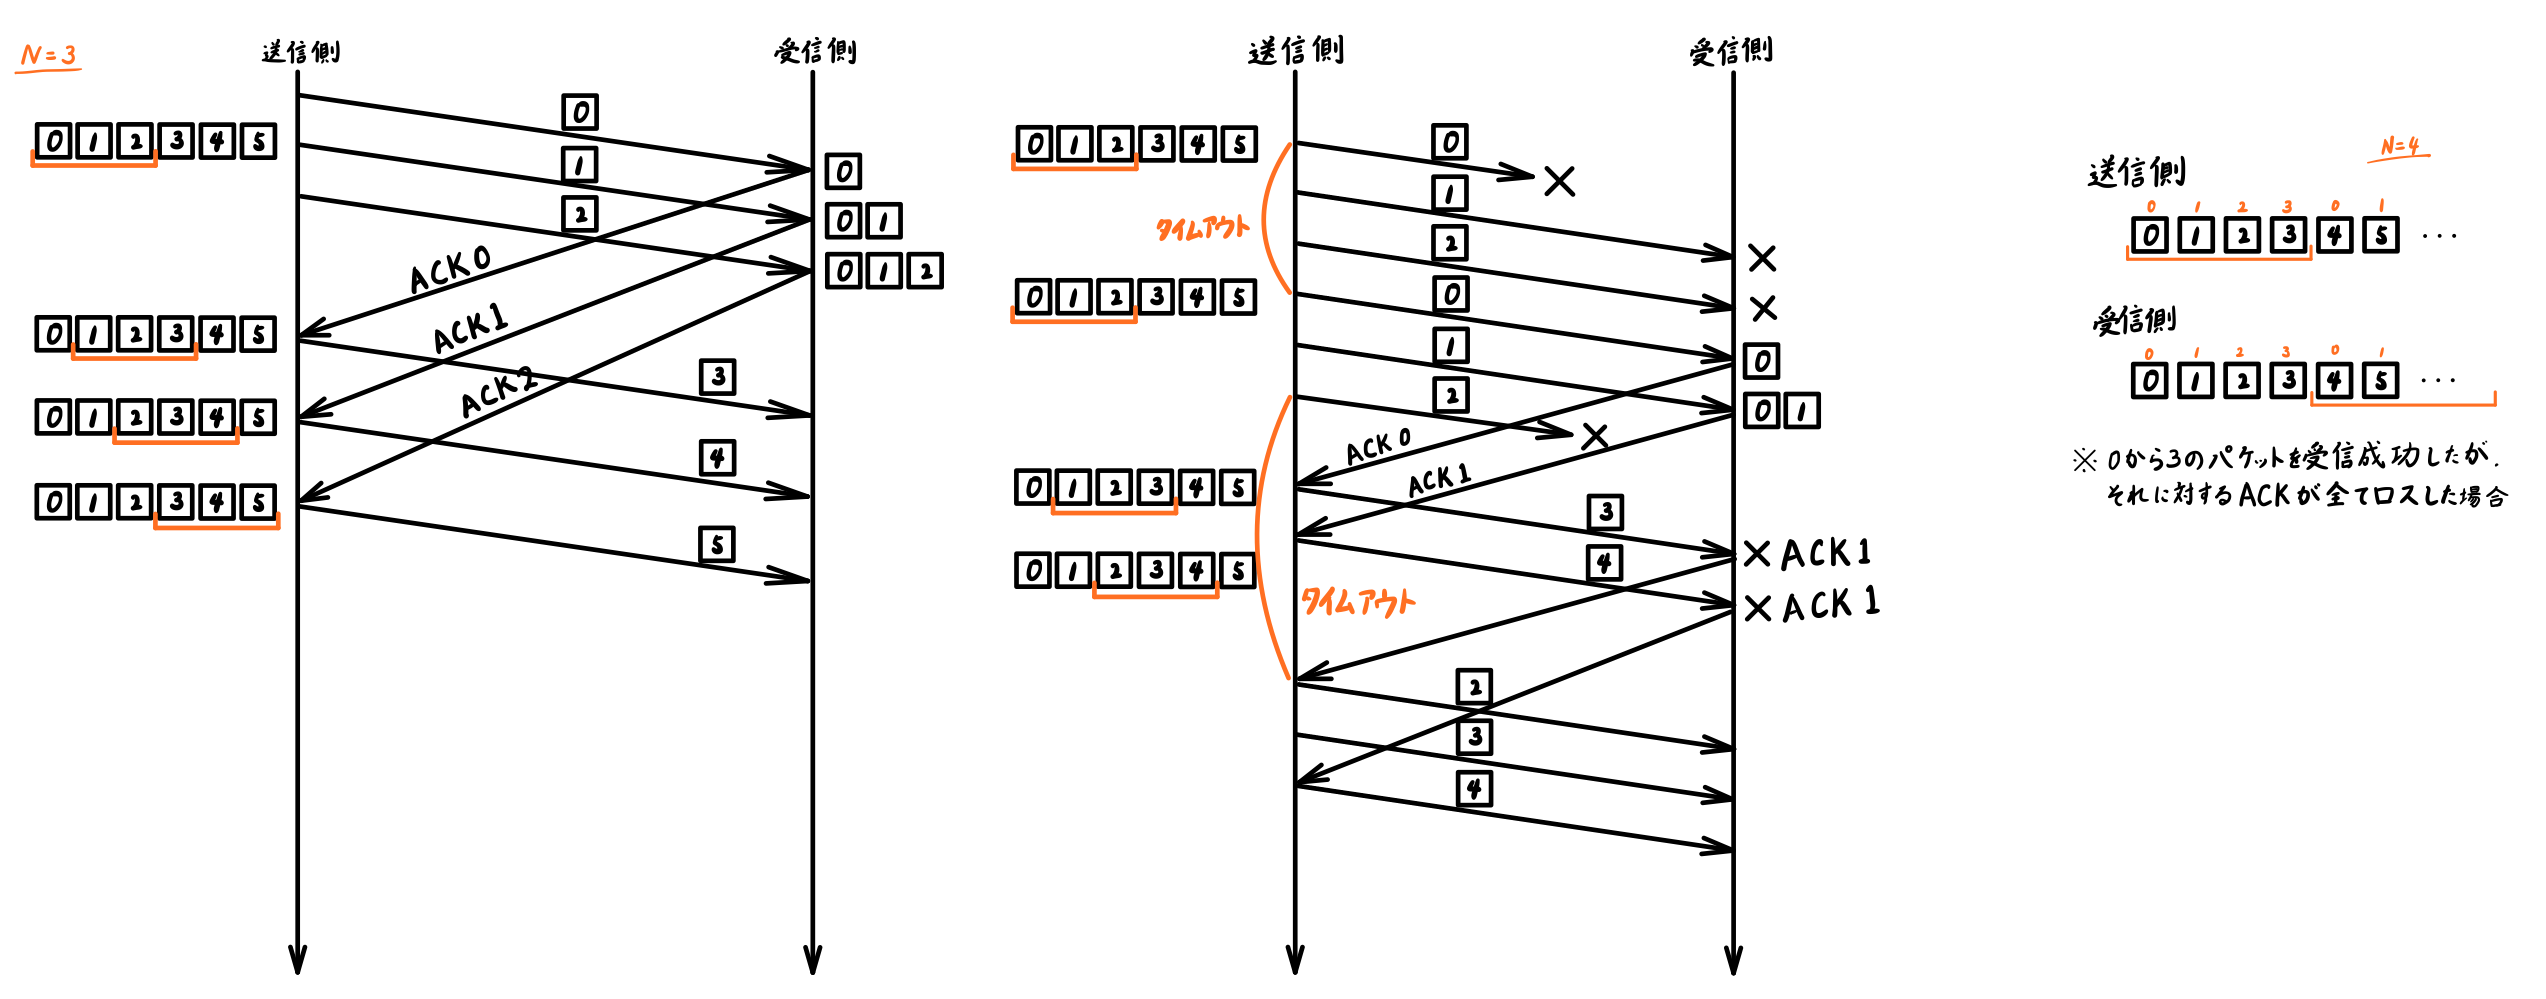
\includegraphics[width=0.9\linewidth]{image/cumulative_ack.png}
\end{figure}

\textcolor{cyan}{gbnの場合はシーケンス番号の方が(パケットサイズもしくはパケットより)1ビット大きくもつ必要がある}

\newpage
\subsubsection{SR (selective-Repeat)}

ACKの受信を待たずに連続するパケットを最大 N 個まで送信可

送信失敗が確認されると、そのパケットのみ再送  (受信バッファサイズ N)

\begin{itemize}
  \item 送信側
  \begin{itemize}
    \item パケットにシーケンス番号を付加 ($k$ ビット)
    \item ウィンドウサイズ (N $\leq 2^{k-1}$) とタイムアウト時間を設定
    \begin{itemize}
      \item n: 送信したが、ACK未受信のパケットの最小シーケンス番号
    \end{itemize}
  \end{itemize}
  \begin{enumerate}
    \item 次に送るべきパケットのうち、 $n+N-1$ 番までを連続的に送信し、2へ
    \item 各パケットに対するACKの受信を待つ
    \begin{enumerate}
      \item タイムアウト時間内にACKを受信したら、1へ
      \item タイムアウト時間内にACKを受信しなければそのパケットを再送し、2へ
    \end{enumerate}
  \end{enumerate}
  \item 受信側
  \begin{enumerate}
    \item パケットを受け取ったら、誤りがないか確認
    \item 誤りがなければ、\undercolor{そのシーケンス番号を付加したACK}
    \footnote{\textcolor{orange}{選択的(Selective) ACK}}
    を送信\\
      (順序通りに上位層へ渡すため、バッファリング)
  \end{enumerate}
\end{itemize}

\begin{figure}[h]
% img: 上記のGo-back-Nの図を編集したもの
% 左側は "SRでも同じ"
% ウィンドウ内のすべてのパケットに対応するACKが返ってきたらウィンドウを移動?
  \centering
  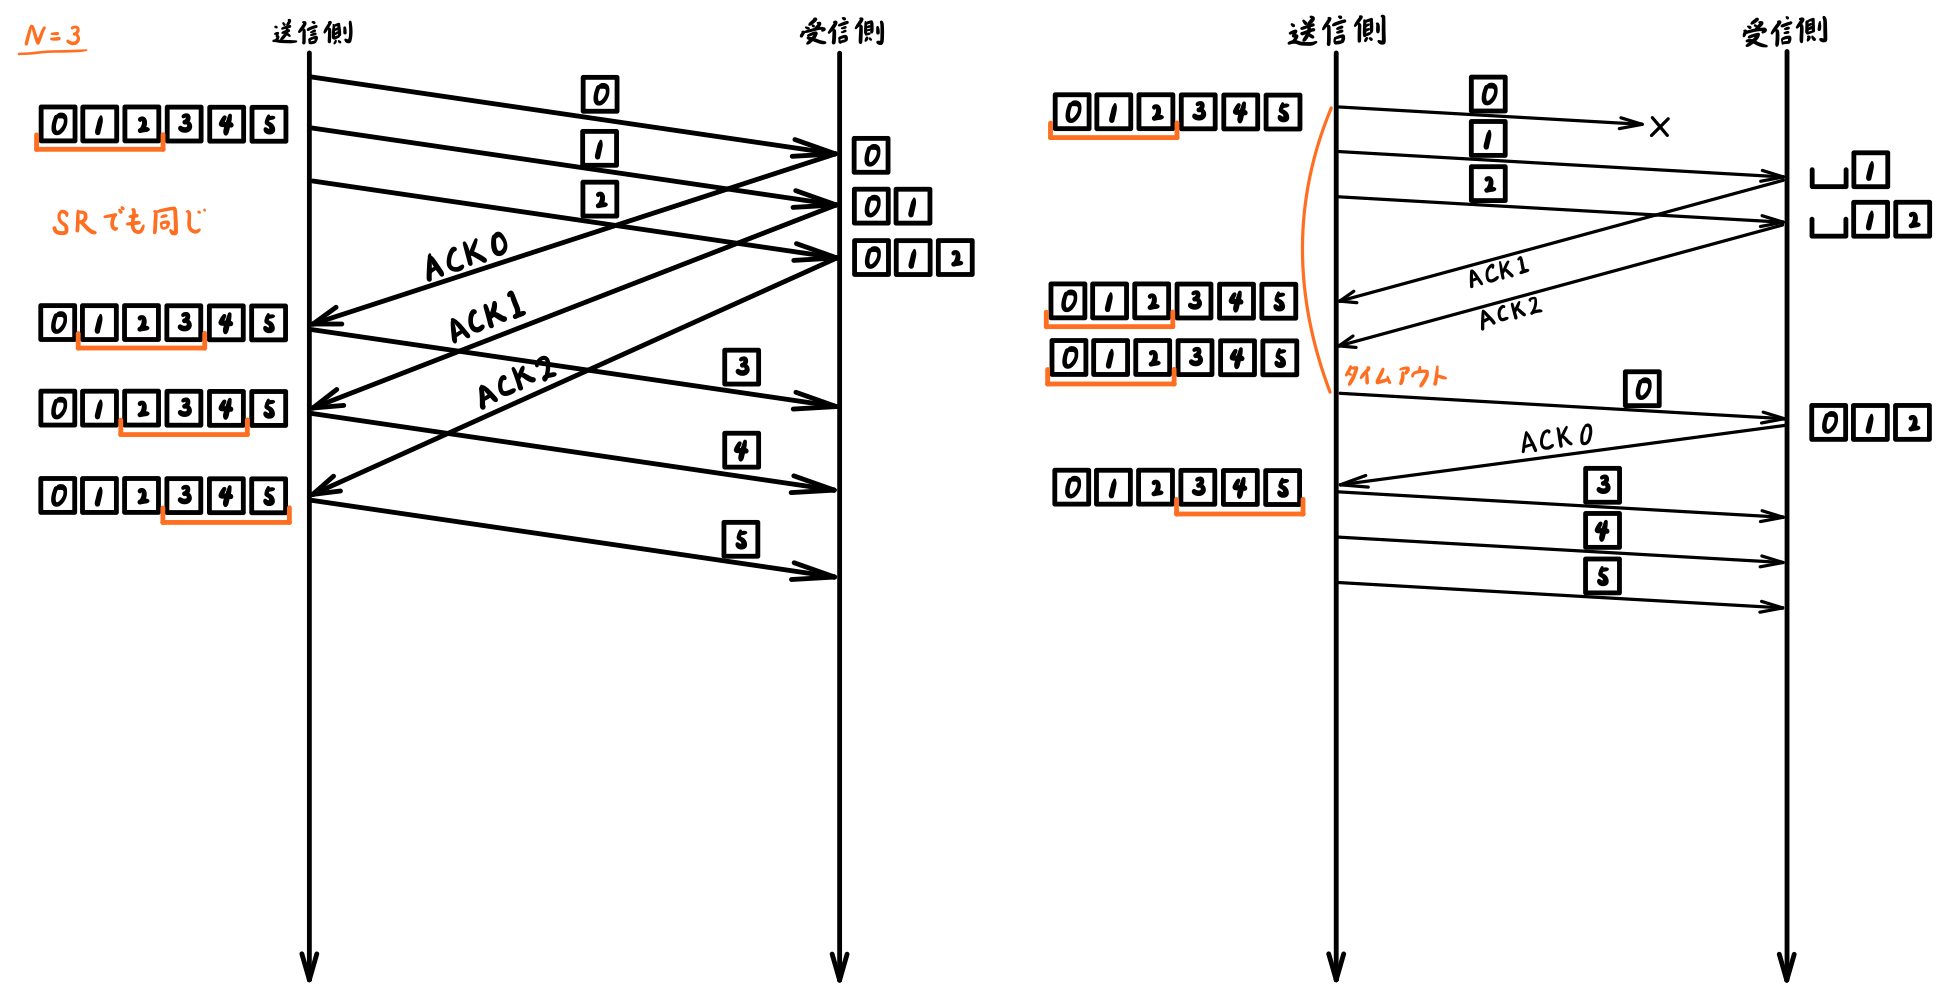
\includegraphics[width=0.8\linewidth]{image/selective_repeat.png}
\end{figure}

% 次回の頭に解説するらしい この手法が有効な場合の例?

% TCPはざっくりGo-back-Nだけど、すぐに捨てるわけじゃないみたい(前回メモ) + 輻輳制御の話に


\end{document}
